\documentclass{beamer}

\usetheme{Warsaw}
\title{Introduction To Programming}
\subtitle{Basic algorithmic thinking}
\author{Rastko Tojagi\' c}

\usepackage[utf8]{inputenc}

\newcommand{\bfemph}[1]{\textbf{#1}}
\renewcommand{\emph}[1]{\bfemph{#1}}

% Defines section title page
\AtBeginSection[]{
  \begin{frame}
  \vfill
  \centering
  \begin{beamercolorbox}[sep=8pt,center,shadow=true,rounded=true]{title}
    \usebeamerfont{title}\insertsectionhead\par%
  \end{beamercolorbox}
  \vfill
  \end{frame}
}

\begin{document}

\maketitle

% \begin{frame}
    %     Ovo je glavni deo dokumenta!
    %     Komanda \verb"\LaTeX" generi\v se
    %     logo: \LaTeX!
% \end{frame}

\section{History}
\begin{frame}
    \frametitle{History}
    The concept of algorithm has existed since antiquity.
    Arithmetic algorithms, such as a \emph{division algorithm}, was used by ancient Babylonian mathematicians c. 2500 BC and Egyptian mathematicians c. 1550 BC.
    
    \bigskip
    
    Greek mathematicians later used algorithms in the \emph{sieve of Eratosthenes}
    for finding prime numbers, and the \emph{Euclidean algorithm} for finding the greatest common divisor of two numbers.
    
\end{frame}

\begin{frame}
    \frametitle{History}
    The word algorithm itself is derived from the 9th-century Persian mathematician Muhammad ibn Ahmad al-Khwarizmi, Latinized \emph{Algoritmi}.
\end{frame}    

\begin{frame}
    \frametitle{History}
    \begin{columns}
        \column{0.6\textwidth}
        \begin{itemize}
            \item 19th century  
            \item Mathematician and writer
            \item First published algorithm
        \end{itemize}
        
        \column{0.35\textwidth}
        \centering
        
        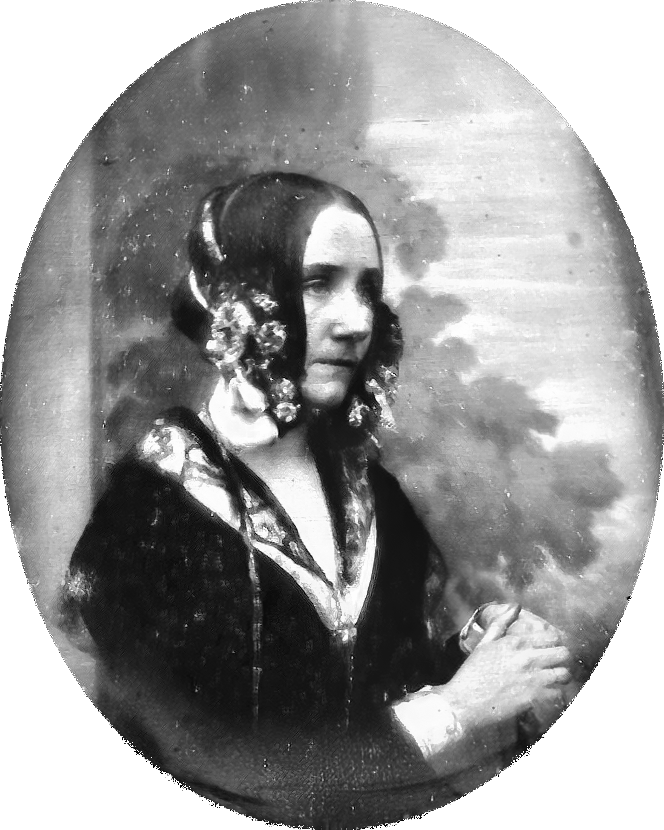
\includegraphics[scale=0.16]{figures/ada.png}
        
        \bigskip
        
        {\scriptsize Augusta Ada King, Countess of Lovelace}
    \end{columns}
    
\end{frame}   

\begin{frame}
    \frametitle{History}
    Ada Lovelace's diagram from "note G", the first published computer algorithm.
    
    \bigskip
    
    \centerline{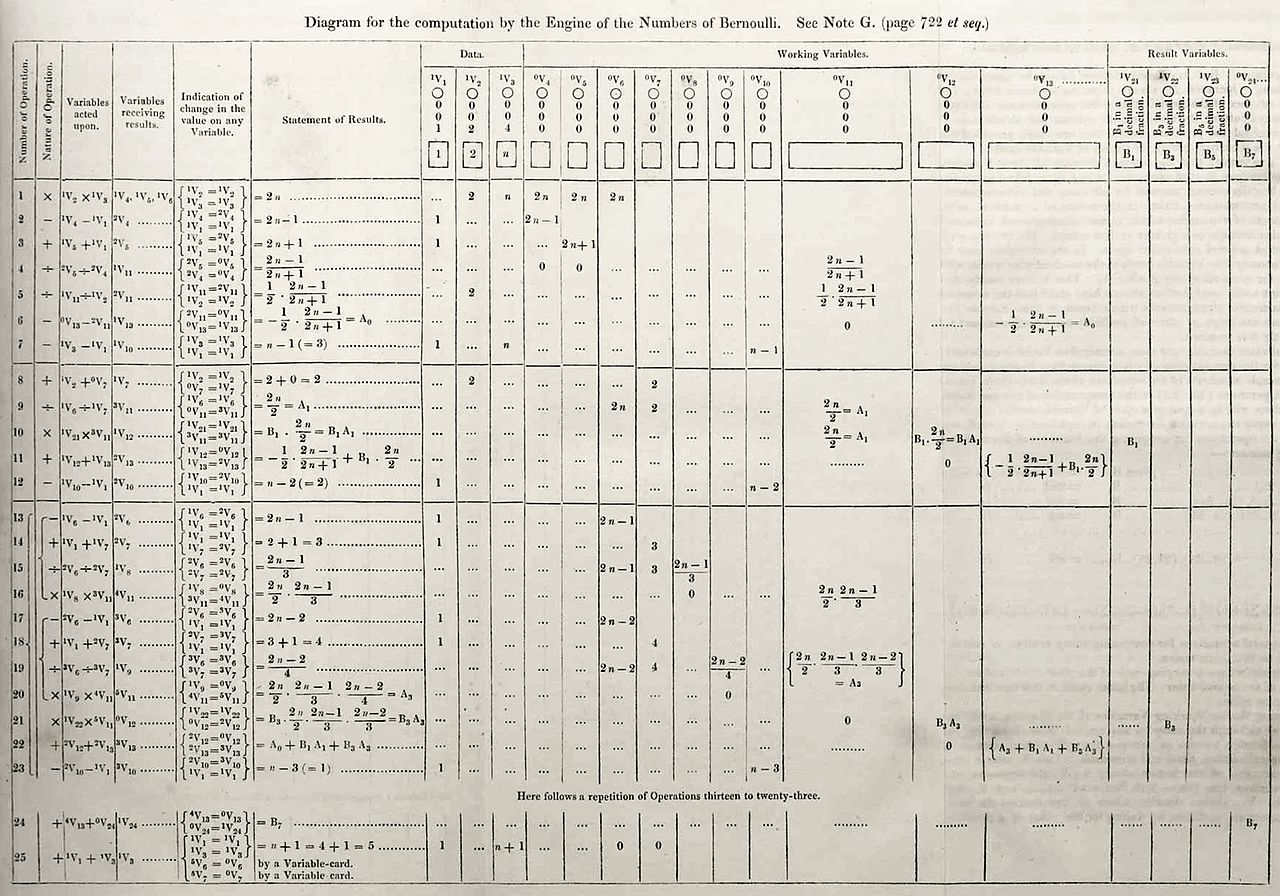
\includegraphics[scale=0.2]{figures/ada_diagram.jpg}}
    
\end{frame}

\section{Algorithms}
\begin{frame}

    \begin{block}{Definition}
        A finite sequence of well-defined (unambiguous) instructions is called an \emph{algorithm}.
    \end{block}

\end{frame}

\end{document}